\chapter{Simulation and Reconstruction}
\label{chap:Reconstruction}

\chapterquote{How to open a pandora box?}%
{A wise Chinese}%: Blackwood's Magazine May 1830

%As previously stated, this document focus on the \ILD and \CLICILD detectors. Due to the similarity, we often only discuss one detector to avoid the repetition. The difference in detectors will be stated if applicable.

In previous chapters, overviews of the theory and the future linear collider experiments have been described. Since the work presented in this document is for future collider, simulation and monte carlo method is used throughout the document. In this chapter, the simulation and event reconstruction chain are discussed, with emphasis on the \pandora event reconstrcution, which provides the background for the photon reconstruction algorithms in \Chapter{chap:Reconstruction}.

Simulation and reconstruction of events for the future Linear Colliders, \ILC and \CLIC, share common software framework. The noticeable difference will be discussed.

\section{Monte Carlo event generation}

For the simulated study, Monte Carlo (MC) event generation is the first step. Most events, electron-positron interaction, are generated with WHIZARD software, \cite{whizard,Moretti:2001zz}, with no polarisation of the electron and positrons. Some simple events are generated with HEPEVT. PYTHIA \cite{Sjostrand:1995iq} is used to describe parton showering, hadronisation and fragmentation. The parameters for PYTHIA are tuned to OPAL data from the LEP \cite{Alexander:1995bk}. TAUOLA \cite{Jadach:1993hs} debrides the tau lepton decay with correct spin correlations of the day products. The Initial State Radiation (\ISR) is simulated in WHIZARD with the \ISR photons being collinear with the beam direction. The Final State Radiation (\FSR) is simulated with default parameters in PYTHIA.

For the \CLIC simulated samples, the luminosity spectrum, which is generated with GUINEAPIG \cite{Schulte:1999tx}, is simulated in WHIZARD. The \ggHad background events are hadronised with PYTHIA, and superimposed on the physics process simulations to save computational resources.

TODO
\ggHad simulation -5 to 25ns etc


\section{Event Simulation}

The event simulation software is GEANT4 \cite{Agostinelli:2002hh}, and the detector geometry description is provided by MOKKA \cite{MoradeFreitas:2002kj}.  QGSP\_BERT physics list is used to describe the hadronic showers decay in the detector.


%Simulation and reconstruction of events for the future Linear Colliders share common software framework. Simulated events are generated with Whizard software \cite{}. Pythia describes hadronisation and Tauola simulates correct spins of tau lepton decay products.  Whizard allows events simulation without initial state radiation, and can simulate electron beam interaction. For the \CLIC detector, electron beam induced background events are simulated and reconstructed. These events are superimposed on the physics process to save computational resources.


\section{Event Reconstruction}

Reconstruction software runs in Marlin framework \cite{Gaede:2006pj}, as a part of the \ilcsoft. Event reconstruction contains following steps: digitisation of simulated calorimeter hits, reconstruction of tracks in the tracking system using pattern recognition algorithms, and particle flow objects (\PFOs)reconstruction with \pandora\cite{Thomson:2009rp,Marshall:2012ry}. Reconstruction does not include calorimeters hits in the forward calorimeters, due to computational reasons  (see \Section{sec:doubleHiggsForwardElectron}).

For the \CLIC detector simulations, suppression of \ggHad background is performed.

Details of the reconstruction can be found in \cite{Brau:2007zza,Linssen:2012hp}. Particle flow reconstruction via \pandora will be discussed in details, which provides the background for the photon reconstructions in \pandora in \Chapter{chap:Reconstruction}.

\section{\pandora}
\label{sec:pandoraPandoraPFA}
Tradition calorimetric approach is unable to meet the mass and energy requirements for the future linear collider. The particle flow approach with \pandora has a proof-of-principle demonstration of its capability to reach required resolution. The particle flow approach also put stringent requirements on the detector design, which is described in \Chapter{chap:Detector}. By associating calorimeter hits to the tracks, around 60\% of the jet energy from charged particles is measured by the tracker, which has a much better resolution than the calorimeter. Small cell sizes of the calorimeters are required to identify hits from different particles. The traditional sum of calorimeter cell energies is replaced by particle flow reconstruction algorithms, a complex pattern recognition problem.  The \pandora algorithm has been developed and used in the \ILC and \CLIC simulation studies.

Started with the \ILD detector concept, \pandora has been adapted to the \CLIC condition and shows its ability to deliver required energy resolutions \cite{Linssen:2012hp}. Recent the code base of the \pandora has been restructured. The core base codes for basic object and memory managements are factorised in the Pandora C++ Software Development Kit\cite{Marshall:2015rfa}. There are over 60 linear collider specific reconstruction algorithms, each aims to address a particular topological in the reconstruction.

In the subsequent paragraphs, the main steps in the \pandora reconstructions are described. The details of the reconstruction can be found in cite{Thomson:2009rp,Marshall:2012ry,Marshall:2015rfa}.

Inputs of \pandora are digitised calorimeter hits and reconstructed tracks. The output are reconstructed particles with four-momenta, Particle Flow Objects (\PFOs).

\subsection{Track selection}
\label{sec:pandoraPandoraTrack}
Tracks from the tracking system are selected based on their topological properties, how likely they are from physical processes, and whether they are consistent with the tracker resolution. Tracks passed the selection are used for the subsequent reconstruction.  Special topologies of tracks are identified, such as when a neutral particle decays or converts into a pair of charged tracks, leaving a ``V0''  shape tracks. This is identified by searching for a pair of tracks originated from a single point. Another topologies include ``kinks'' , when a charged particle decays to a single charged particles with neutral particles, and ``prongs'', when a charged particles decays to multiple charged particles. This information are stored and passed on to the subsequent reconstruction, along side with the helical track fit (using last 50 reconstructed hits) and the track projection to the front of the \ECAL.

\subsection{Calorimeter selection}

The input information of a calorimeter hit is the position, the layer in the calorimeter and the energy response from the calorimeter.

Calorimeter hits are selected based on a series of criterion. The selected hits need to have energies above the threshold, using the conversion of a minimum ionising particle (MIP) equivalent, and using directly the converted energy. Similar to tracks, only calorimeter passed the selection are used in later steps.

Geometry information and likelihood of the hit originated from a minimum ionising particle (MIP) are calculated.

Isolated hits, often originated from low energy neutrons in a hadronic shower, are difficult to associate to the correct hadronic shower. They are identified and not used in the clustering. But their energy is added in the very last particle flow object (PFO) creation step.

\subsection{Cone Clusters Algorithm}
\label{sec:pandoraConeCluster}
Before discussing the rest of the \pandora reconstruction, it is necessary to introduce the cone based clustering algorithm, which is widely used in the calorimeter in \pandora. The clustering algorithm produces basic working objects, \clusters.


\begin{figure}[tbph]
\centering
{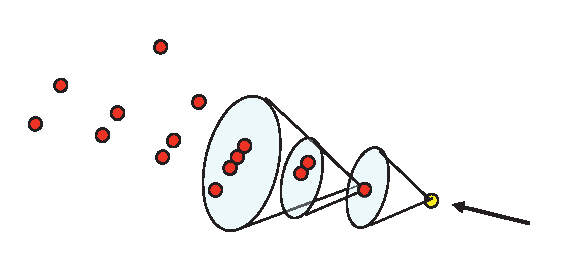
\includegraphics[width=0.5\textwidth]{pandora/coneClustering}}%
\caption{Illustration of the cone clustering algorithm, taken from \cite{Marshall:pandoraLC}}
\label{fig:pandoraConeClustering}
\end{figure}

There are two main types of clustering algorithms: cone based and sequential combination (see \Section{}). The main clustering scheme \pandora is cone clustering, for grouping calorimeter hits. Illustrated in \Figure{fig:pandoraConeClustering}, cone clustering has a specified opening angle of the seed hit. Because the direction of particle flows is largely unchanged from the originated particle, whether it is a electromagnetic shower, QCD radiation or hadronisation, these cone clusters have similar direction and energy to the originated particle. Therefore it is applicable to use cone based clustering algorithms for building clusters.

The seed for the cone clustering is typically the projection of a energetic track to the front of the \ECAL. A high  energy calorimeter hit can also be used as a seed. A cone with a specified opening angle and depth will be formed around the seed. The \fourMomentum of calorimeter hits sum to the cone's \fourMomentum.

TODO
Build from inner to outer, then every layer outer in inner see Mark's paper

\subsection{Particle Identification}
\label{sec:particleID}

Dedicated particle identification algorithms aim to identify muons and photons before associating calorimeter hits to tracks. The details of the photon reconstruction algorithms and photon related algorithms are described in \Chapter{chap:Reconstruction}. By removing the hits from muons and photons, the reconstruction of charged particles is improved as it reduce the pattern recognition problem. Identified muons and photons do not participate in the clustering and re-clustering stages, but re-entre the construction at the fragment removal stage (see \Section{sec:pandoraFragmentRemoval}).

\subsection{Clustering}

The cone clustering algorithm described in \Section{sec:pandoraConeCluster} is used to group calorimeter hits from innermost to outmost pseduo-layer. The output \clusters are further processed, merged or split based on their topological properties.

\subsection{Topological cluster association}

Initial clustering scheme is aggressive at splitting clusters. Small clusters are merged  based on clear topological signatures. These merging signatures include combining track segments, connecting tack segments with gaps, connecting track segment to a hadronic shower, and merging clusters when they are within close proximity.

\subsection{Track-cluster association}

Clusters are associated to tracks, according to the proximity of the first layer of the cluster and the track projection to the front of the \ECAL.


\subsection{Re-clustering}

The cluster association scheme work well for low energy (less than 50\,GeV) jet. For a high energy jet, particles and the subsequent hadronic showers are more boosted and more likely to overlap each other. Therefore, it is important to re-cluster based on the compatibility of the cluster energy and the associated track momentum. A cluster may be split into two. Two clusters maybe be re-clustered based on the track-cluster association. The re-clustering algorithm is applied iteratively to find a more correct clustering of calorimeter hits.

\begin{comment}
\subsection{Photon identification}

The neutral clusters are tested against an expected photon electromagnetic shower profile. The longitudinal shower profile for a photon cluster is required to be similar to a expected electromagnetic shower profile, with the discrepancy being smaller than a threshold.
\end{comment}

\subsection{Fragment removal}
\label{sec:pandoraFragmentRemoval}
The late stage of the reconstruction will focus on merging low energy clusters, especially non-photon neutral clusters. These neutral clusters are likely to be fragments of charged clusters, instead of being a physical particle. The merging criterion are mostly based on the proximity and the energy comparison.

One algorithm will attempt to split up photon clusters, where each is originated from two close by photons. Photon related algorithms are described in details in \Chapter{chap:Reconstruction}.



\subsection{Particle Flow Object Creation}
\label{sec:pandoraPFOcreation}

% double counting taking care in pandora
Particle Flow Objects (PFOs) are created at the last step. Tracks are associated to the clusters based on the proximity. Simple but effective particle identification for electrons, muons are applied. Photon identifications have been applied at various stages of the reconstruction.

PFOs are the output of the \pandora reconstruction. The four-momentum of these PFOs are  used heavily for the downstream analysis. The electron, muon and photon identification are  also used in physics analysis, such as one described in \Chapter{chap:Tau}.

\section{MC truth linker}
Hits contribution to MC particle.
Main contributed MC particle from energy weighted hits
Main contributed Jets etc. from hits
\section{\CLIC specific simulation and reconstruction}



\section{Luminosity spectrum}



\section{Suppression of \ggHad backgrounds}
\label{sec:pandoraggHad}


For the CLIC, significant \ggHad background is present. It is crucial to remove the beam induced background as they don't represent the underlying physics process.

Two Marlin process has been developed to suppress these background, a track selector and a PFO selector\cite{Marshall:2012ry}.

The track selector aims to remove poor quality and fake tracks. It places simple quality cut and a simple time of arrival cut. If the arrival time of the track at the front of the \ECAL, using the helical fit, differs more than 50\,ns from using a straight line fit, the track will be rejected.

The PFO selector utilise the high spatial resolution from the high granular calorimeter. PFOs from \ggHad often have low \pT and have a range of time. PFOs from physics processes have a range of \pT, and have time close to the brunch crossing time. These two distinctive features allow \ggHad background to be separated. The optimal suppression uses different \pT and time cuts for the central part of the detector, and for the forward part of the detector, and uses different cuts for photons, neutral PFOs and charged PFOs. Three configurations of these cuts are developed, namely ``loose'', ``normal'', and ``tight'' selections. As the name suggested, ``loose'' selection corresponds to a looser cut of \pT and time. The optimal configuration depends on the \sqrtS of the collision, and the physics process to study.

The background suppression is used in analysis described in \Chapter{chap:DoubleHiggs}
TODO add efficiency table pandora
TODO add timing pT cut and table of energies

\section{\CLIC simulated particle masses} 